\documentclass[../../main.tex]{subfiles}
\graphicspath{{\subfix{../../images/}}}

\begin{document}

    \subsection{Warstwa użytkownika - frontend}

    \subsubsection{Wstęp}
    Warstwa użytkownika została zrealizowana przy użyciu frameworka Angular, który umożliwia szybkie tworzenie dynamicznych i responsywnych aplikacji webowych w języku TypeScript. Angular dostarcza zaawansowane narzędzia do zarządzania stanem aplikacji, budowania komponentów wielokrotnego użytku oraz implementacji nawigacji i dynamicznych interfejsów użytkownika.
    Aplikacja komunikuje się z warstwą systemową poprzez REST API, wysyłając żądania HTTP i odbierając odpowiedzi w formacie JSON. Obsługuje również integrację z usługą Amazon Cognito w celu autoryzacji i uwierzytelniania użytkowników, wykorzystując tokeny dostępu JWT.
    Dzięki integracji z Cognito, aplikacja umożliwia logowanie i zarządzanie sesjami użytkowników w sposób bezpieczny i zgodny z OAuth2. Przekierowywanie użytkownika do widoków chronionych odbywa się na podstawie posiadania poprawnego tokenu.
    Komunikacja z zasobami w Amazon S3 (np. przesyłanie lub pobieranie plików) odbywa się przy wykorzystaniu predefiniowanych adresów URL (pre-signed URLs), które są generowane przez backend. Dzięki temu frontend nie ma bezpośredniego dostępu do zasobów w S3, co podnosi bezpieczeństwo aplikacji.
    Dzięki zastosowaniu Angulara i TypeScript warstwa użytkownika jest modularna, łatwa w utrzymaniu oraz zorientowana na dostarczenie intuicyjnego i płynnego doświadczenia dla użytkownika końcowego.

    \subsubsection{Struktura plików}
    Warstwa użytkownika została zaimplementowana przy pomocy frameworku Angular\cite{angular} opartego o język TypeScript (TS). Strukturę plików przedstawia Rysunek \ref{fig:frontend-repo-structure}.

    \begin{figure}[ht!]
        \begin{subfigure}{.5\textwidth}
            \centering
            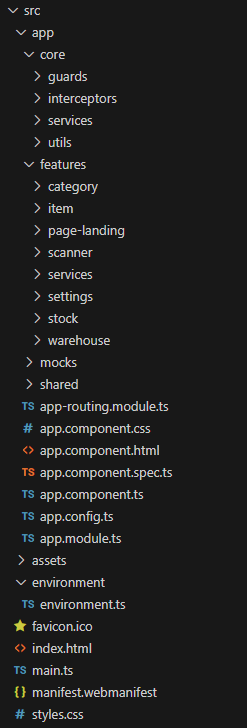
\includegraphics[height=0.4\pdfpageheight]{images/front-repo-structure.png}
            \caption{Ogólna struktura plików}
            \label{fig:front-repo-structure-general}
        \end{subfigure}
        \begin{subfigure}{.5\textwidth}
            \centering
            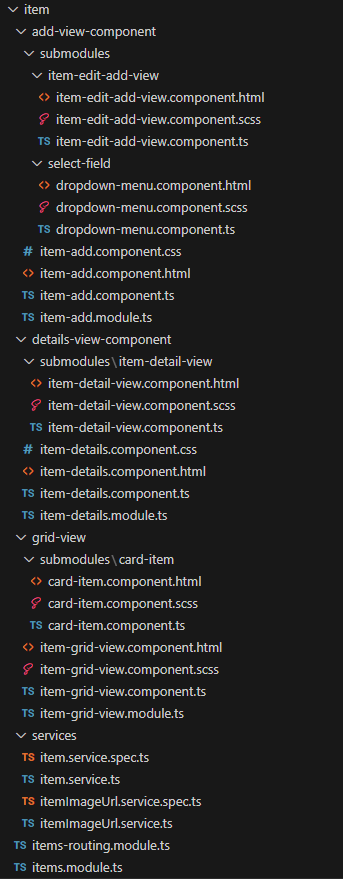
\includegraphics[height=0.4\pdfpageheight]{images/frontend-repo-structure-feature.png}
            \caption{Dokładna struktura jednego z komponentów}
            \label{fig:front-repo-structure-feature}
        \end{subfigure}
        \caption{Struktura plików frontendu}
        \label{fig:frontend-repo-structure}
    \end{figure}

    Aplikacja jest tworzona przy pomocy komponentów. Każdy komponent składa się ze skryptu TS, pliku stylu SCSS oraz pliku układu HTML. Dodatkowo niektóre komponenty korzystają z serwisów napisanych w języku TypeScript. 

    \begin{itemize}
        \item \textbf{app} - folder, w którym znajduje się prawie cała logika aplikacji
        \begin{itemize}
            \item \textbf{core} - przechowywane są w nim serwisy, interceptory i guardy. Kod, który używany jest w całej aplikacji
            \begin{itemize}
                \item \textbf{guards} -  guardy za pomocą których kontrolowany jest dostęp użytkowników do poszczególnych stron. 
                \item \textbf{interceptors} - interceptory pozwalają przechwytywać i modyfikować żądania oraz odpowiedzi HTTP. 
                \item \textbf{services} - serwisy do obsługi ról użytkowników (definiujące dostęp do funkcjonalności) oraz serwis obsługujący cognito
                \item \textbf{utils} - serwis, za pomocą którego zdjęcia są odpowiednio cachowane
            \end{itemize}
            \item \textbf{features} - folder, w którym umiejscowione są konkretne implementacje poszczególnych widoków
            \begin{itemize}
                \item \textbf{category} - konkretne implementacje poszczególnych widoków dotyczących kategorii
                \item \textbf{item} - konkretne implementacje poszczególnych widoków dotyczących produktów
                \item \textbf{page-landing} - konkretna implementacja widoku dotyczącego strony startowej
                \item \textbf{scanner} - konkretna implementacja widoku dotyczącego strony ze skanerem
                \item \textbf{services} - implementacja serwisu z którego korzystam w poszczególnych widokach do obsługi localstorage
                \item \textbf{settings} - konkretna implementacja widoku dotyczącego strony z ustawieniami
                \item \textbf{stock} - konkretne implementacje poszczególnych widoków dotyczących stanu magazynów
                \item \textbf{warehouse} - konkretne implementacje poszczególnych widoków dotyczących magazynów
            \end{itemize}
            \item \textbf{mocks} - folder, w którym przechowuje się klasy modeli wykorzystywane do testowania
            \item \textbf{shared} - komponenty graficzne zazwyczaj wykorzystywane wiele razy: strony z błedami oraz podkomponenty używane w wielu widokach  
        \end{itemize}
        \item \textbf{assets} - folder, w którym znajdują wykorzystane zasoby w aplikacji
        \begin{itemize}
            \item \textbf{logo} - folder, w którym są umieszczone loga o różnych rozmiarach potrzebne do stworzenia manifestu potrzebnego do działania PWA
            \item \textbf{icons} - folder, w którym są przechowywane ikony wykorzystane podczas tworzenia aplikacji
        \end{itemize}
        \item \textbf{environment} - folder, w którym znajduje się environment.ts - plik ze zdefiniowanymi zmiennymi środowiskowymi
    \end{itemize}

    \subsubsection{Widoki}
    Warstwa wizualna tworzona jest za pomocą rozszerzonego przez Angular HTML. Styl definiowany jest za pomocą plików SCSS - rozszerzonym CSS. Widoki są tak zaprojektowane w taki sposób, aby oznaczały się wygodą użytkowania oraz odpowiednią skalownością na różnych rozmiarach ekranów, bez znaczenia czy są to urządzenia mobilne, czy komputery sacjonarne. 

    \subsubsection{Routing}
    Ścieżki w aplikacji frontendowej są zabezpieczone poprzez ekstrakcję ról z tokenu JWT, który kontroluje dostęp do zasobów, zapewniając, że tylko autoryzowani użytkownicy z odpowiednimi uprawnieniami mają dostęp do określonych widoków.

    \subsubsection{Testy}
    Testy obejmują wszystkie serwisy, zapewnia to poprawność działania aplikacji w różnych scenariuszach, w tym przypadkach brzegowych i błędnych, w celu zapewnienia niezawodności i bezpieczeństwa. %tylko nie localstorage xD

    \subsubsection{Konteneryzacja - Docker}
    Aplikacja frontendowa została skonteneryzowana za pomocą Dockera, co pozwala na łatwe uruchomienie aplikacji w izolowanym środowisku kontenerowym:

    \begin{itemize}
        \item Plik \texttt{Dockerfile} wykorzystuje wieloetapowe budowanie, optymalizując proces tworzenia obrazu. Dzięki temu obraz jest lekki i zawiera tylko niezbędne zależności.
        Na pierwszym etapie (cache) pobierane są zależności z plików \texttt{package.json} i \texttt{package-lock.json} i cache’owane, co przyspiesza kolejne kompilacje.
        Na drugim etapie (builder) aplikacja jest kompilowana za pomocą Angular CLI i polecenia \texttt{ng build}, tworząc statyczne pliki w katalogu \texttt{/app/dist}, gotowe do serwowania przez Nginx.
        Na ostatnim etapie (runner) uruchamiana jest aplikacja na lekkim obrazie \texttt{nginx:1.27.0-alpine3.19}, który serwuje pliki statyczne, z domyślnie wystawionym portem 80. Skrypt \texttt{run.sh} uruchamia proces Nginx w trybie deamon.
        \item Plik \texttt{compose.yml} umożliwia uruchomienie aplikacji frontendowej na maszynie lokalnej w celach deweloperskich, testowych lub produkcyjnych.
        \item Plik \texttt{nginx.conf} definiuje konfigurację serwera Nginx, który będzie serwował pliki statyczne aplikacji frontendowej.
        \item Plik \texttt{nginx.conf.template} jest szablonem konfiguracji Nginx, wykorzystywanym przez Docker'a.
        \item Plik \texttt{env.template} zawiera nazwy zmiennych środowiskowych, które są wymagane do uruchomienia aplikacji.
        \item Plik \texttt{.dockerignore} ogranicza kontekst budowania obrazu, ignorując zbędne pliki, co przyspiesza proces budowania obrazu.
    \end{itemize}
    Całość konfiguracji pomaga oraz umożliwia szybkie, niezawodne i powtarzalne uruchamianie aplikacji w kontenerach, co pozwala na łatwe testowanie i rozwijanie aplikacji w różnych środowiskach.

\subsubsection{Inne}
W celu zaimplementowania funkcji wyboru lokalizacji użytkownika oraz lokalizacji magazynu w aplikacji wykorzystano bibliotekę Leaflet\cite{leaflet} w połączeniu z danymi mapowymi dostarczanymi przez OpenStreetMap\cite{openstreetmap}. Leaflet jest lekkim i wszechstronnym narzędziem do pracy z mapami interaktywnymi, co pozwoliło na intuicyjne i dynamiczne zarządzanie lokalizacjami w aplikacji. Aby upewnić się, że wskazana lokalizacja użytkownika jest poprawna wykorzystani dostęp do lokalizacji urządzenia. 

W aplikacji wdrożono funkcję umożliwiającą szybki dostęp do informacji na temat przechowywanego produktu w magazynie poprzez skanowanie kodów QR lub kodów kreskowych EAN. Ta funkcjonalność znacząco przyspiesza procesy wyszukiwania produktów oraz zarządzaniem stanem magazynowym.

\end{document}